\section{Miscellaneous Notes}
% the text width in a normal line is 11.80737cm
% To make a TODO note, start a comment with two or more consecutive capital letters.

% Figures are in the gfx folder. They should not have dots in the names
% since that interferes with the crossref function. They should be named
% something like '01-intro.png' where the first two digits are the 
% chapter number and then some simple description of the figure.

% Potential arrangement (for 2nd ed???): 
%		3 Background chapters
%		8 Chapters about ``Traditional'' procedures
%		4 Chapters about Business Analytics, datamining, etc.

% TODO
% Add whatever graphics I can to each chapter
% Add example research reports

% Use an ``Objective'' box for objectives and ``Summary'' box for summary. Both boxes are found below. Chapters 1 and 11 have an objectives box at the top and a summary box at the end. Use either as a guide for other chapters.


%******************************************************
\section{3-Line Equation}
%******************************************************
\begin{align}
	\label{03:eq:identity_example}
	1101_2 &= 123 \\
	\nonumber
	&= 123 \\
	\nonumber
	&= 123
\end{align}


\section{Solving an Equation Step-by-step}
\begin{align}
	\label{04:soln:solving_equation_one}
	AB+BC(B+C) && \text{Original Expression} \\
	\nonumber
	AB+BBC+BCC && \text{Distribute BC} \\
	\nonumber
	AB+BC+BC && \text{Idempotence: BB=B and CC=C} \\
	\nonumber
	AB+BC && \text{Idempotence: BC+BC=BC} \\
	\nonumber
	B(A+C) && \text{Factor} \\
\end{align}

%**************************************************************************
\section{Margin Paragraph} 
%**************************************************************************
% Use to create a sidebar paragraph out in the margin
\marginpar{Whatever.}

%**************************************************************************
\section{Footnote Without Marker} 
%**************************************************************************
% Use to create a footnote without a numbering marker
\blfootnote{Whatever.}

%***************************************************************************
\section{Text Box}
%***************************************************************************
% Creates a nice boxed text with a title and main section
\begin{tcolorbox}[colback=blue!5!white,colframe=blue!75!black]
	% Upper half of box: my "title" area
	\textcolor{blue}{\textbf{Interesing Note}}
	% Lower half of the box: the content
	\tcblower
	Whatever.
\end{tcolorbox}

%***************************************************************************
\section{Objectives Box}
% Relies on ``objbox'' in config file
%***************************************************************************
\begin{center}
	\begin{objbox}{Objectives}
		\begin{itemize}
			\setlength{\itemsep}{0pt}
			\setlength{\parskip}{0pt}
			\setlength{\parsep}{0pt}
		
			\item x1.
			\item x2.
			\item x3.
		\end{itemize}
	\end{objbox}
\end{center}

%***************************************************************************
\section{Takeaway Box}
% Relies on ``tkawybox'' in config file
%***************************************************************************
\begin{center}
	\begin{tkawybox}{Ch Title}
		\begin{itemize}
			\setlength{\itemsep}{0pt}
			\setlength{\parskip}{0pt}
			\setlength{\parsep}{0pt}
				
			\item x1.
			\item x2.
			\item x3.
		\end{itemize}
	\end{tkawybox}
\end{center}

%**********************************************************************
\section{Text Table}
%**********************************************************************
\begin{table}[H]
	\centering
	\begin{tabulary}{\linewidth}{LCCCC}
		\hline
		\multicolumn{5}{l}{\textbf{Do you support these propositions?}} \\
		\hline
		Prop & Strongly Support & Support & Do Not Support & Strongly Do Not Support  \\ 
		\hline
		100 & $\bigcirc$ & $\bigcirc$ & $\bigcirc$ & $\bigcirc$ \\ 
		115 & $\bigcirc$ & $\bigcirc$ & $\bigcirc$ & $\bigcirc$ \\ 
		220 & $\bigcirc$ & $\bigcirc$ & $\bigcirc$ & $\bigcirc$ \\ 
		\hline
	\end{tabulary} 
	\caption{My great table.}
	\label{03:tab01}
\end{table}


%**********************************************************************
\section{Text Table: Default for this document}
%**********************************************************************
\begin{table}[H]
	\rowcolors{1}{}{tablerow} % zebra striping background
	{\small
		%\fontsize{8}{10} \selectfont %Replace small for special font size
		\begin{longtable}{
				L{0.15\linewidth}
				L{0.15\linewidth}
			} %Left-aligned, Max width: 4.25in
			% \multicolumn{2}{c}{\textbf{Header 1}}\\
			\textbf{ColA} & \textbf{ColB} \endhead
			\hline
			A & B\\
			W & X\\
			\rowcolor{captionwhite}
			\caption{Caption}
			\label{01:tab01}
		\end{longtable}
	} % End small
\end{table}

%***************************************************************************
\section{ToDo}
%***************************************************************************
% Create a ToDo note in the text. This also creates a new clickable TODO
% section in the ``structure'' box on the left side of the page.
%TODO This is a todo note.

%***************************************************************************
\section{Code Snip}
%***************************************************************************
\lstset{ %
  caption={caption},
  label=SL:lst:listing01,
  numbers=left,
  language=Verilog
}
\begin{lstlisting}
  Code here
\end{lstlisting}

%***************************************************************************
\section{Introductory Figure}
%**************************************************************************
% Use this for figures at the top of each chapter

\begin{wrapfigure}{r}{0.4\textwidth}
	\centering
	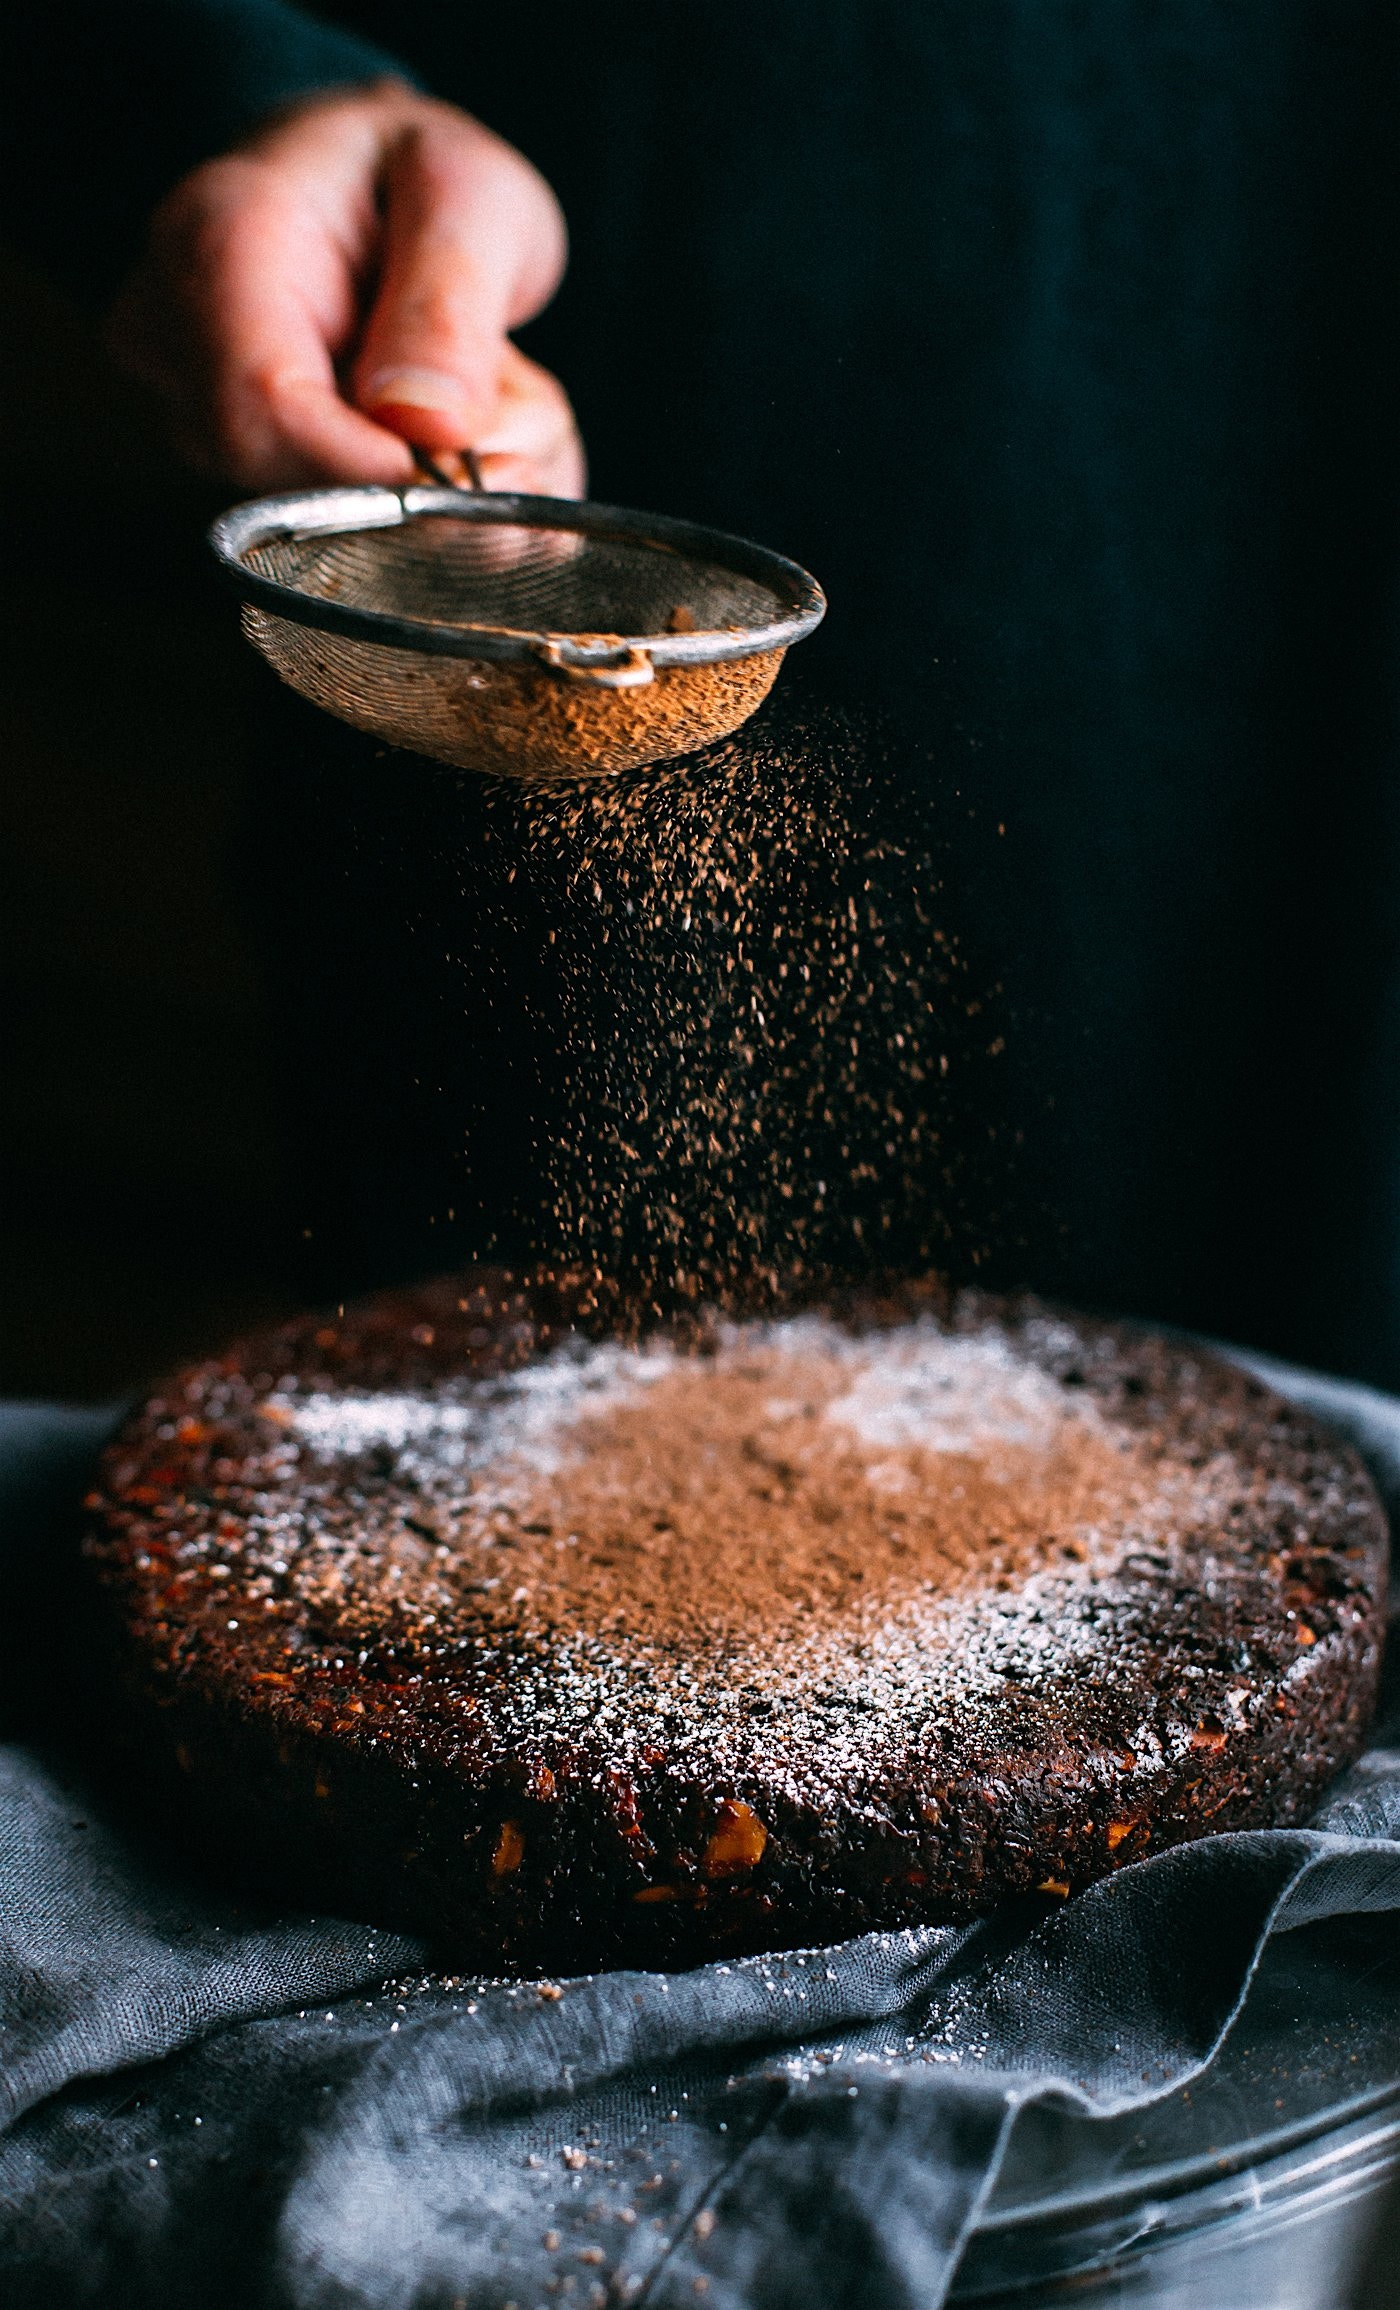
\includegraphics[width=0.4\textwidth]{gfx/05-cake} 
\end{wrapfigure}

First paragraph.\blfootnote{Photo by lindsay Cotter on Unsplash}

%***************************************************************************
\section{Wrap Figure}
%**************************************************************************
\begin{wrapfigure}{O}{0.2\textwidth}
	\caption{} % No text, wraps badly in very narrow space (does print fig number)
	% to not print a fig number use \caption*{}
	\label{03:fig02} 
	\centering
	
\includegraphics[width=0.2\textwidth]{gfx/99-placeholder} 
\end{wrapfigure}


%***************************************************************************
\section{Sampling of Research}
%**************************************************************************
\noindent\begin{minipage}{\textwidth}
	\begin{figure}[H]
		\centering
		
\includegraphics[width=.85\linewidth]{gfx/Sampling_Of_Research}
		\caption*{}
		\label{01:sampling_of_research}
	\end{figure}
	\vspace{-10.0ex} %Note: neg 10 heights of letter x
	\section{A Sampling of Research}
\end{minipage}
\subsection{Report Title}



%***************************************************************************
\section{Regular Figure}
%**************************************************************************
\begin{figure}[H]
	\centering
	
\includegraphics[width=\maxwidth{.95\linewidth}]{gfx/99-placeholder}
	\caption{Caption}
	\label{03:fig03}
\end{figure}



%***************************************************************************
\section{Lorem}
%**************************************************************************
Lorem ipsum dolor sit amet, consectetuer adipiscing elit. Aenean commodo ligula eget dolor. Aenean massa. Cum sociis natoque penatibus et magnis dis parturient montes, nascetur ridiculus mus. Donec quam felis, ultricies nec, pellentesque eu, pretium quis, sem. Nulla consequat massa quis enim. Donec pede justo, fringilla vel, aliquet nec, vulputate eget, arcu. In enim justo, rhoncus ut, imperdiet a, venenatis vitae, justo. Nullam dictum felis eu pede mollis pretium. Integer tincidunt. Cras dapibus. Vivamus elementum semper nisi. Aenean vulputate eleifend tellus. Aenean leo ligula, porttitor eu, consequat vitae, eleifend ac, enim. Aliquam lorem ante, dapibus in, viverra quis, feugiat a, tellus. Phasellus viverra nulla ut metus varius laoreet. Quisque rutrum. Aenean imperdiet. Etiam ultricies nisi vel augue. Curabitur ullamcorper ultricies nisi. Nam eget dui. Etiam rhoncus. Maecenas tempus, tellus eget condimentum rhoncus, sem quam semper libero, sit amet adipiscing sem neque sed ipsum. Nam quam nunc, blandit vel, luctus pulvinar, hendrerit id, lorem. Maecenas nec odio et ante tincidunt tempus. Donec vitae sapien ut libero venenatis faucibus. Nullam quis ante. Etiam sit amet orci eget eros faucibus tincidunt. Duis leo. Sed fringilla mauris sit amet nibh. Donec sodales sagittis magna. Sed consequat, leo eget bibendum sodales, augue velit cursus nunc,

%***************************************************************************
\section{Style Guide}
%**************************************************************************

For menu selections:
Click \textsc{\fbox{Analyze $ \rightarrow $ Descriptive Statistics $ \rightarrow $ Frequencies}}

Labels should be a chapter, colon, verbal desc (all lc with underscores): \label{03:title}
For figures, label should be chapter, colon, ``fig'' and number: \label{03:fig01}

Dates do not include an apostrophe: In the 1960s this happened...

Wrap all numbers in an in-line math block: $ 123 $

The word ``data'' is plural, thus: ``Data are analyzed...''